\documentclass[11pt]{article}
\usepackage{amsmath,amsthm,verbatim,amssymb,amsfonts,amscd, graphicx}
\usepackage{graphicx}
\usepackage{subcaption}
\usepackage{listings}
\usepackage{float}
\usepackage{url}
\usepackage{titlesec}
\setcounter{secnumdepth}{4}


\graphicspath{{./times/}}
\topmargin0.0cm
\headheight0.0cm
\headsep0.0cm
\oddsidemargin0.0cm
\textheight23.0cm
\textwidth16.5cm
\footskip1.0cm

\titleformat{\paragraph}
{\normalfont\normalsize\bfseries}{\theparagraph}{1em}{}
\titlespacing*{\paragraph}
{0pt}{3.25ex plus 1ex minus .2ex}{1.5ex plus .2ex}


\begin{document}
\title{CS 5220\\ Comparative Study on the Computational Speed Between Skylines and Pardiso Sparse Direct Solver}
\author{Marc Aurele Gilles (mtg79)\\ Wenjia Gu (wg233)\\Wensi Wu(382) }
\maketitle

\section{Introduction}\label{sec:intro}

The goal of this project was to compare the performance of two different sparse direct solvers. First, we took a look at our in-house quasi-static structural code, $3D\_geom\_nonlin\_truss.c$. The numerical implementation of the code is described in section \ref{sec:method}.  The $3D\_geom\_nonlin\_truss.c $ is a geometrically nonlinear finite element code embedded with the feature of analyzing truss structures using skyline indexing scheme and compact Gaussian elimination strategy, active column solution or the skyline reduciton method, to solve a large system of equations. In section \ref{sec:setup}, we describe the two different input structures we used for the performance analysis.  A detailed description of the skyline indexing scheme is provided in section \ref{sec:originalCode}. \\

The solver in which we compared our original code with is the MKL sparse solver: Pardiso. Pardiso has features of solving large symmetric and nonsymmetric linear systems of equaitons, $AX=B$, using a parallel $LU$, $LDL^T$ or $LL^T$ factorization where $L$, $U$, and $D$ are the low triangle, upper triangle and the diagonal of matrix $A$ respectively. The solver employes parallel pivoting methods based on OpenMP directives, which result in the robust and memory-efficient performance. In section ~\ref{sec:newCode} we will describe how we translated the skyline indexing scheme in the original code into Compressed Sparse Row (csr) format in order to take advantage of the Pardiso solver.\\

After we successfully hooked Pardiso into our original code, we conducted weak and strong scaling studies for both sparse direct methods. The results can be found in section \ref{sec:scaling}.  


\section{Numerical Method}

The truss computing problem can be written in the form
$$F_l(u)=0$$
where u is the displacement, and F is a system of $n$ non-linear equations, where n depends on the number of nodes, elements and degrees of freedom(?), and l is the maximum load factor.

We solve this system of equation using a continuation method, starting at $l=0$, and incrementally increasing $l$ until it reaches the user specified maximum $l^{\star}$. 
\\
Each $F_l(u)=0$ equation is solved by a Newton method iteration.

That is we repeatedly solve $F_l(u_{t+1}) \simeq F_l(u_t) + S_l(u_t)*u_{t+1} =0$, where $S_l(u_t)$ is the Jacobian matrix at $u_t$, which in this problem is the same as the Stiffness matrix. 
In other words, each iteration is a linear solve:
$$S_l(u_t)*u_{t+1}=-F_l(u_t)$$.

Most of the computation of this program is spent doing this linear solve. The stiffness matrix for large structures is very high dimensional and very sparse, a sparse solver is therefore needed.

\section{Setup: generating input structures}

As our objective is to speed up this computation and conduct scaling studies, we need to be able to generate input structures of variable sizes.
We wrote two scripts that generate two different type of input structures, a "chain" structure (see figure ~\ref{fig:chain}) , and a "pyramid" structure (see figure ~\ref{fig:pyramid}) .


\begin{figure}[h]
\begin{center}

\caption{A chain structure of 7 elements}
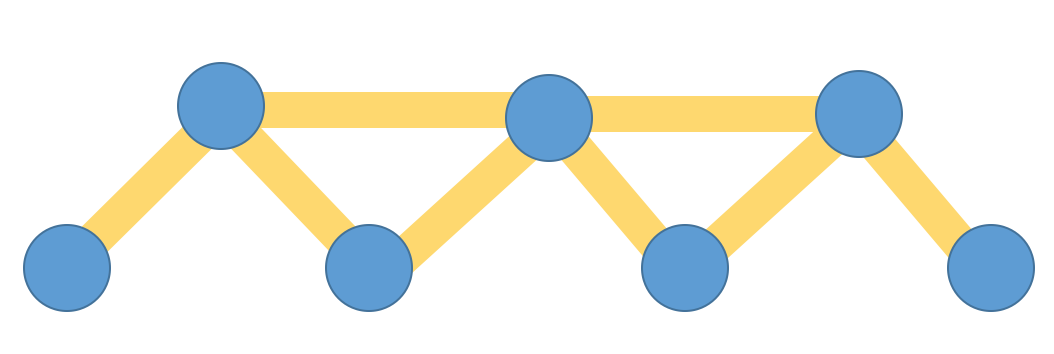
\includegraphics[width=8cm]{chain}
\label{fig:chain}
\\
The blue circles are the nodes, and the yellow bars are the elements
\end{center}

\end{figure}


\begin{figure}[h]
\begin{center}

\caption{A pyramid structure of 6 elements}
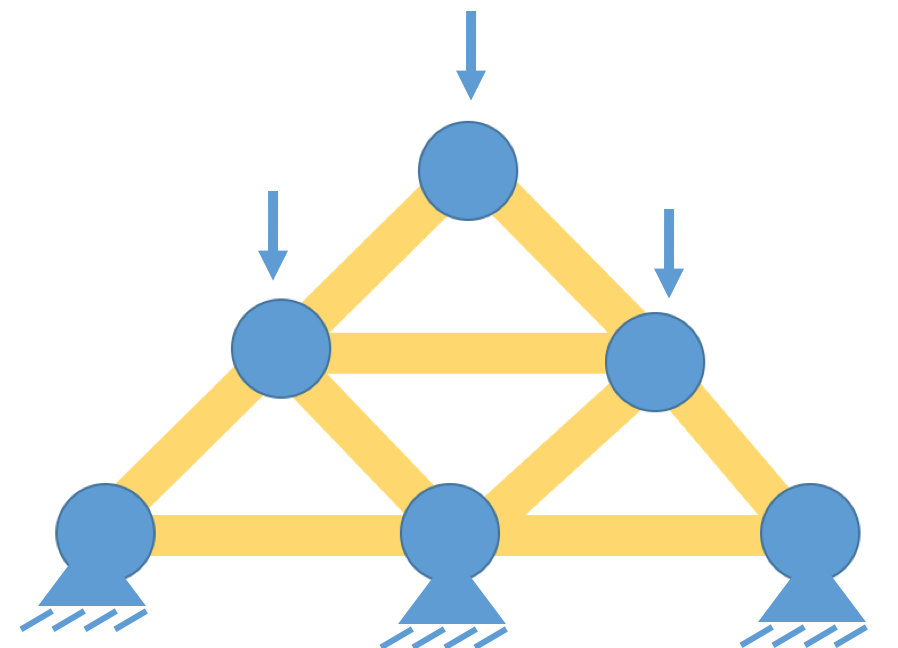
\includegraphics[width=8cm]{pyramid}
\label{fig:pyramid}
\\
The blue circles are the nodes, and the yellow bars are the elements
\end{center}

\end{figure}



For each structure we declare the position of each node, the position of each elements (as defined by a pair of nodes), the properties of each element (cross section area and the corresponding young's modulus ), and a load factor on each node.

These two different structure give rise to significantly different running time and sparsity patterns in the stiffness matrix, for a fixed number of elements. Indeed, the chain structure produces a stiffness matrix with a small dense band, which is not the case for the pyramid structure.

\begin{figure}[H]
\begin{center}
\caption{Sparsity structure of the stiffness matrix generated from the pyramid structure}
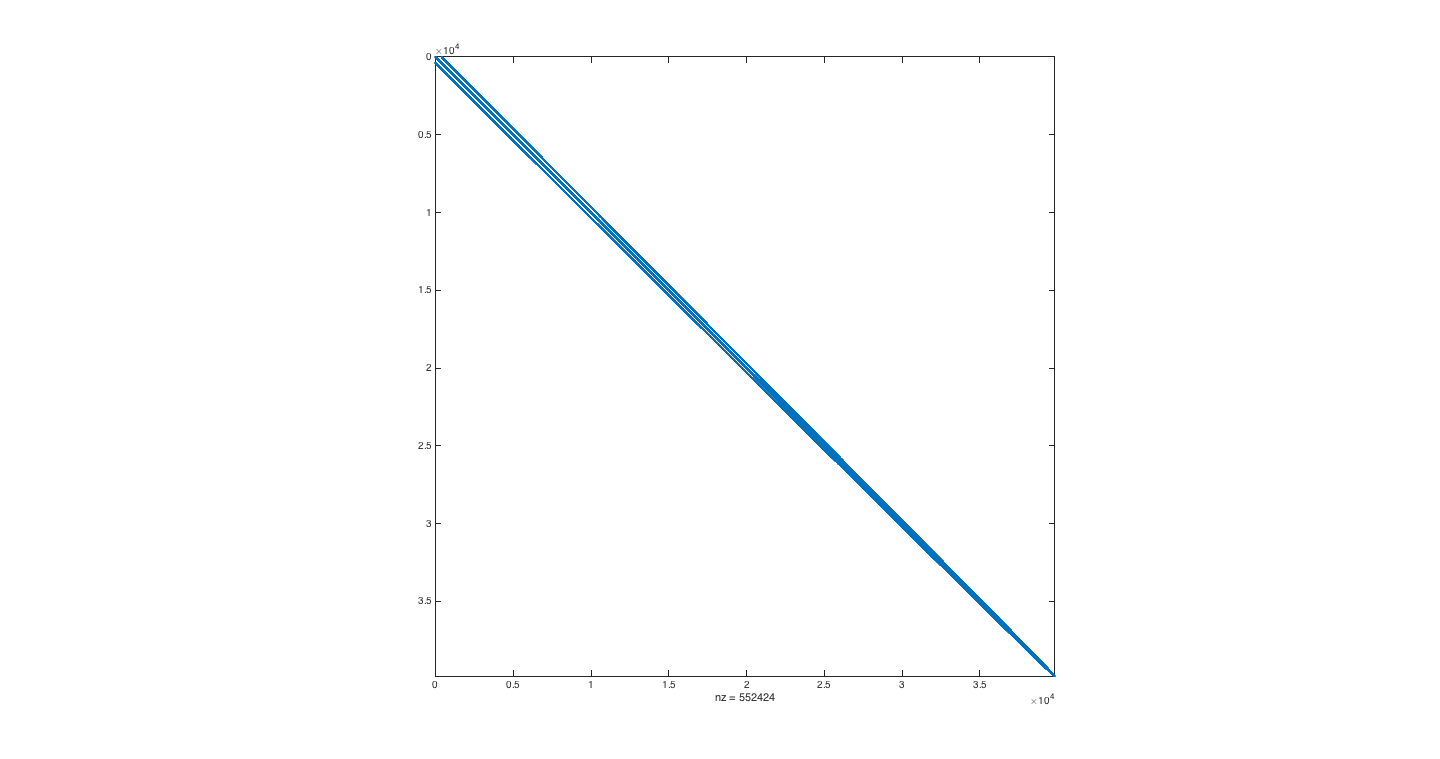
\includegraphics[width=20cm]{pyramid-sparsity.png}
\label{fig:pyramid-sparsity}
\\
\end{center}

\end{figure}

\section{Original code}
The original code reads in all of the parameter of the structure, and performs numerical method described above. At each iteration it generates the stiffness matrix (the Jacobian), and uses a linear solve that takes advantage of the sparsity pattern of the matrix. The matrix storage format is Skyline indexing (described below). The solver takes advantage of the regular access of the skyline indexing to perform a fast Cholesky-like factorization of the form $LDL^T$ (put source here and stuff). The original code is serial.


\subsection{Skyline}
Skyline is a sparse indexing format widely used in finite element codes for structural mechanics. A matrix in skyline format is two arrays: 
\begin{enumerate}

\item a value array which contains the values of the values between the "skyline" and the diagonal
\item a  pointer array for which the ith elements points to the index in the entry in the value array which contains the first non zero element in column i, and the last element is the size of the value array (+1 in case of the fortran-style indexing).

\end{enumerate}

\begin{figure}[h]
\begin{center}

\caption{Example of a matrix stored in skyline format}
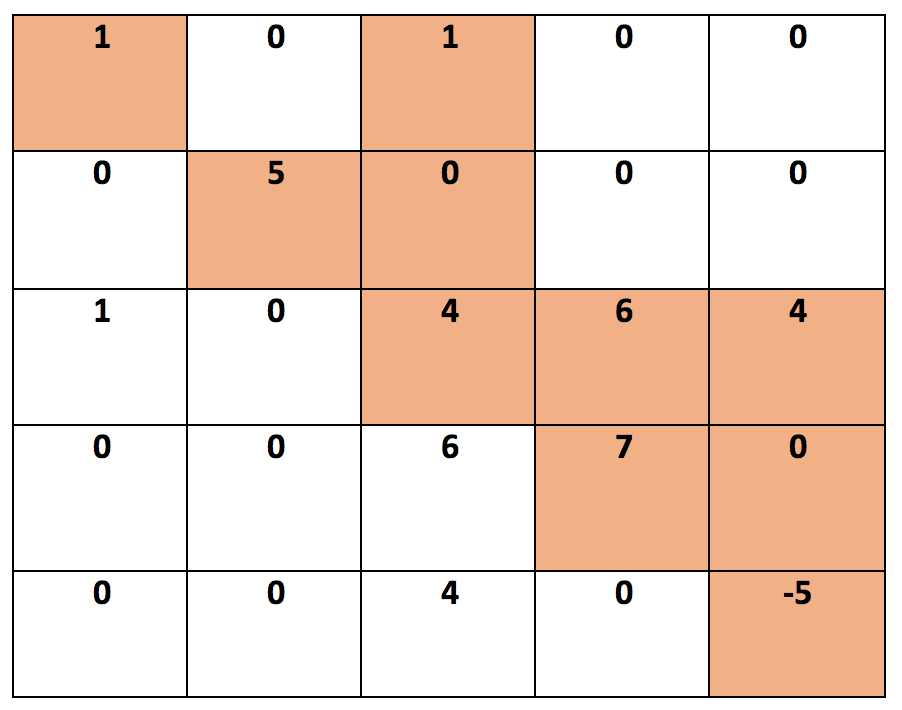
\includegraphics[width=8cm]{skyline}
\label{fig:skyline}
\\
The blue slots are the skyline (stored), and the orange are the other elements stored in the skyline matrix format
\end{center}

\end{figure}
The matrix above in skyline format would be:

\begin{align}
values&=[1,5,1,0,4,6,7,4,0,-5]\\
pointers&= [1,2,3,6,8,11] 
\end{align}
Note that this uses the fortran style 1-based indexing

 It takes advantage of the fact that matrices that arise in this field are usually banded, symmetric positive definite matrices. Solving the system with such a matrix is usually (like in our code) by doing a sparse Cholesky-like decomposition. What makes the skyline indexing attractive is that the fill happening during the decomposition is only within the "skyline".
Though the skyline format is usually very efficient for small systems, it is known that the format can be less than ideal in bigger systems, where the "band" of the matrix grows large, and becomes itself  sparse.


\subsection{Timing of original code}

Below is the relevant part of a result of a timing of the original code on the test case of pyramid with size of base 200 using amplxe.
\begin{center}
 \begin{tabular}{||c c c ||} 
 \hline
 Function & Description & CPU Time \\ [0.5ex] 
 \hline\hline
 solve & Sparse linear solve & 32.560s  \\ 
 \hline
 intel memset  & allocates memory & 0.273s  \\
 \hline
 printf fp & prints to file & 0.132s  \\
 \hline
 stiff & computes stiffness matrix & 0.104s  \\
 \hline
  forces & computes residual forces & 0.078s  \\[1ex] 
 \hline
\end{tabular}
\end{center}

It is clear that most of the time is spent in the function solve, which performs the sparse linear solve, therefore we focused on using a more efficient sparse solver.


\subsection{Vectorization of original code}
On top of introducing sparse direct solver to the original code, we thought of vectorizing the solve function to ensure that it was efficient enough. As shown in the vectorization report (see figure \ref{fig:vectorization}), the solve function was already vectorize based on the report. As a result, we didn't have to do much on vectorization. 

\begin{figure}[H]
	\begin{center}
		
		\caption{Vectorization report of the solve function}
		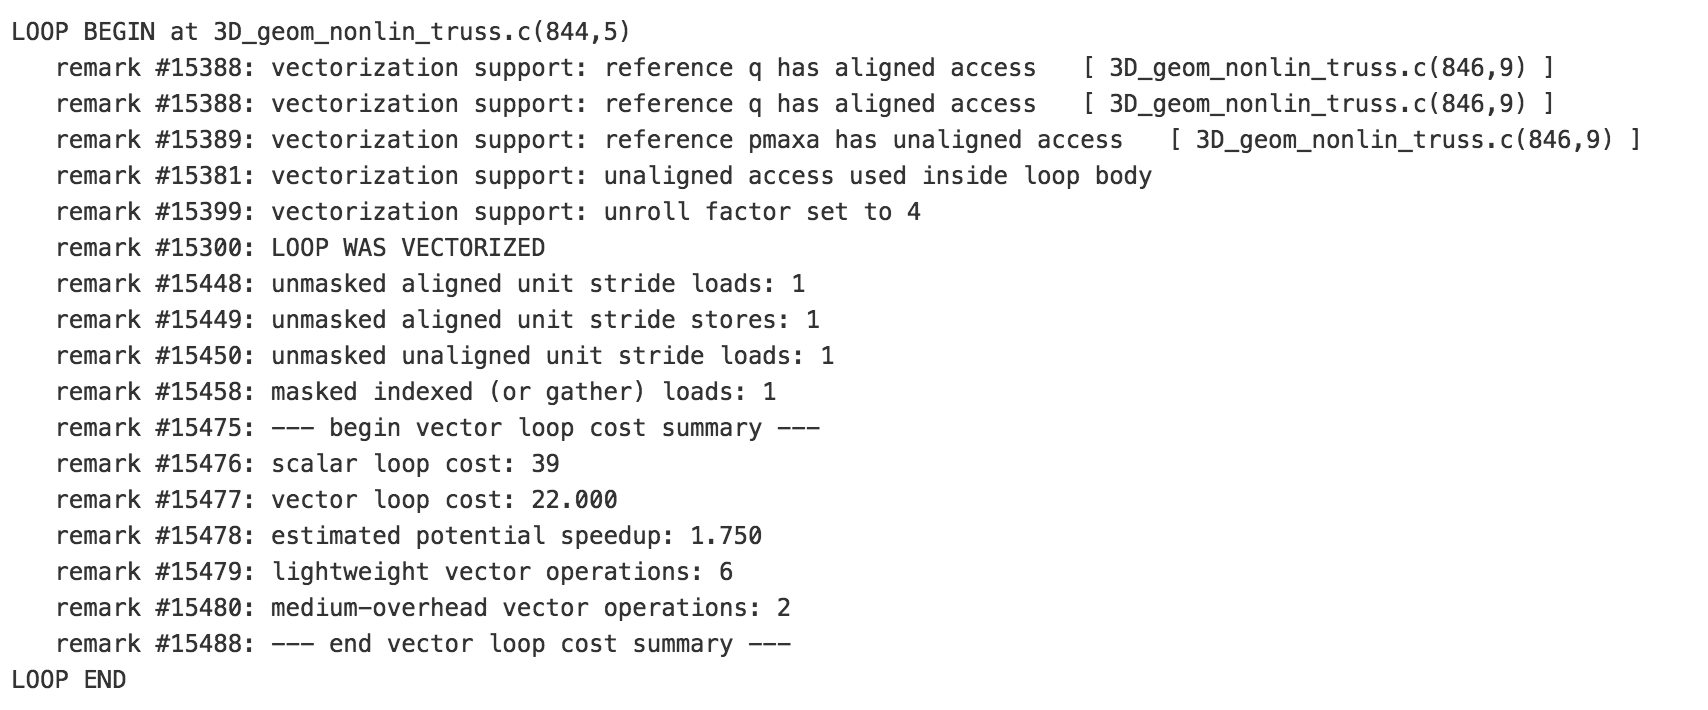
\includegraphics[width=12cm]{vectorization}
		\label{fig:vectorization}
	\end{center}
	
\end{figure}


\section{New code}
Our new code translates the skyline format into a Compressed Sparse Row (csr) format and then uses the MKL parallel sparse solver: pardiso. On the test case 

\subsection{Compressed sparse row}

Compressed Sparse Row (CSR)format is the most common sparse indexing format in scientific computing. A matrix in CSR format constitutes of three arrays:
\begin{enumerate}
\item the value array which contains the non-zero elements of the matrix
\item the column pointer array, where element i is the number of the column in A that contains the i-th value in the values array
\item the row array, where the element j of this integer array gives the index of the element in the values array that is first non-zero element in a row j of A
\end{enumerate}
Note that since pardiso a symmetric solver, we only need to solve the upper triangular part of the matrix
\begin{figure}[H]
\begin{center}
\caption{Example of a matrix stored in CSR format}
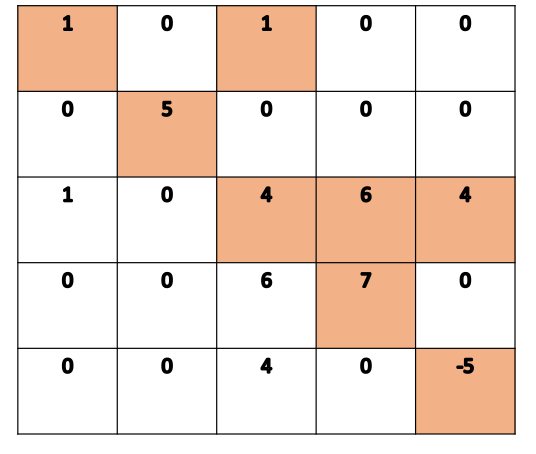
\includegraphics[width=8cm]{csr}
\label{fig:csr}\\
The entries in orange are the entries saved in the symmetric CSR format
\end{center}
\end{figure}

The matrix above in skyline format would be:

\begin{align}
values&=[1,1,5,4,6,4,7,-5]\\
columns&= [1,3,2,3,4,5,4,5] \\
rows&= [1,3,4,7,8,9] 
\end{align}

\subsection{Pardiso}
\subsection{Timing comparisons}
Below is a figure showing  the comparisons of running time between the original solver and the pardiso solver with standard settings on the chain structure. \\

We observe that on the chain structure, both solver are very fast (about 1 second for a structure with 30.000 elements, but the original solver is slightly better. This is likely due to the fact that the original solver is very efficient on this system generated by the structure. Indeed as observed earlier the stiffness matrix in this case have a small but dense band, which is where the solver using the skyline format excels.


\begin{figure}[H]
\begin{center}

\caption{Comparison of running time on pyramid structures}
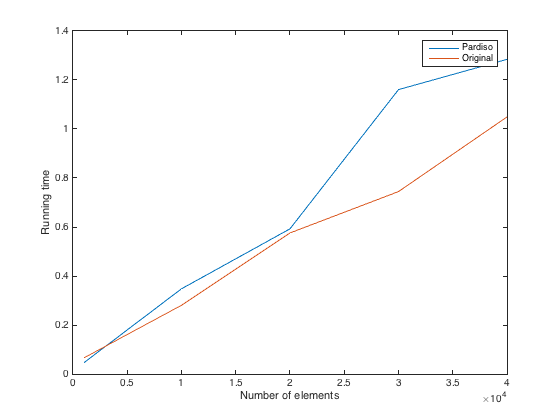
\includegraphics[width=12cm]{chainplot}
\label{fig:pyr_comp}
\end{center}
\end{figure}

Below is a figure showing  the comparisons of running time between the original solver and the pardiso solver with standard settings on the pyramid structure. \\

Contrary to the chain structure, on the pyramid structure the pardiso solver is much faster. This is likely due to the fact that the skyline format keeps a very high number of zeros, and therefore performs a lot of unnecessary arithmetic. Indeed, for the case where we have a 40.000, over $98\%$ of the entries saved by the skyline format are zeros.


\begin{figure}[H]
\begin{center}

\caption{Comparison of running time on pyramid structures}
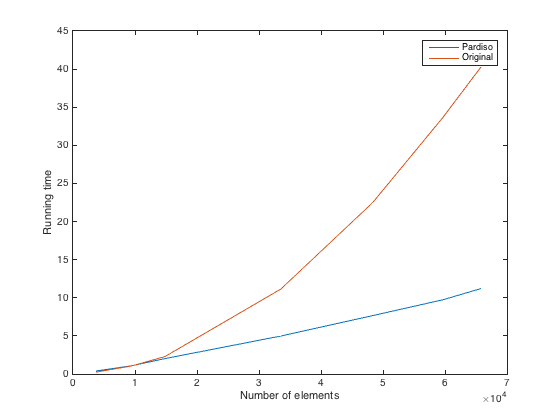
\includegraphics[width=12cm]{pyrplot}
\label{fig:pyr_comp}
\end{center}
\end{figure}



\section{Scaling studies}

\section{Conclusion}

\end{document}